%%%%%%%%%%%%%%%%%%%%%%%%%%%%%%%%%%%%%%%%%%%%%%%%%%%%%%%%%%%%%%%%%%%%%%%%%%%%%
%% Original default rstudio/pandoc latex file
%% upated by @jhollist 09/15/2014
%% inspired by @cboetting https://github.com/cboettig/template and
%% @rmflight blog posts:
%% http://rmflight.github.io/posts/2014/07/analyses_as_packages.html
%% http://rmflight.github.io/posts/2014/07/vignetteAnalysis.html).
%%%%%%%%%%%%%%%%%%%%%%%%%%%%%%%%%%%%%%%%%%%%%%%%%%%%%%%%%%%%%%%%%%%%%%%%%%%%%

\documentclass[11pt,a4paper]{article}
\usepackage[T1]{fontenc}
\usepackage{lmodern}
\usepackage{amssymb,amsmath}
\usepackage{ifxetex,ifluatex}
\usepackage{fixltx2e} % provides \textsubscript
% use upquote if available, for straight quotes in verbatim environments
\IfFileExists{upquote.sty}{\usepackage{upquote}}{}
\ifnum 0\ifxetex 1\fi\ifluatex 1\fi=0 % if pdftex
  \usepackage[utf8]{inputenc}
\else % if luatex or xelatex
  \ifxetex
    \usepackage{mathspec}
    \usepackage{xltxtra,xunicode}
  \else
    \usepackage{fontspec}
  \fi
  \defaultfontfeatures{Mapping=tex-text,Scale=MatchLowercase}
  \newcommand{\euro}{€}
\fi
% use microtype if available
\IfFileExists{microtype.sty}{\usepackage{microtype}}{}
\usepackage[margin=1in]{geometry}
\usepackage{longtable,booktabs}
\usepackage{graphicx}
% Redefine \includegraphics so that, unless explicit options are
% given, the image width will not exceed the width of the page.
% Images get their normal width if they fit onto the page, but
% are scaled down if they would overflow the margins.
\makeatletter
\def\ScaleIfNeeded{%
  \ifdim\Gin@nat@width>\linewidth
    \linewidth
  \else
    \Gin@nat@width
  \fi
}
\makeatother
\let\Oldincludegraphics\includegraphics
{%
 \catcode`\@=11\relax%
 \gdef\includegraphics{\@ifnextchar[{\Oldincludegraphics}{\Oldincludegraphics[width=\ScaleIfNeeded]}}%
}%
\ifxetex
  \usepackage[setpagesize=false, % page size defined by xetex
              unicode=false, % unicode breaks when used with xetex
              xetex]{hyperref}
\else
  \usepackage[unicode=true]{hyperref}
\fi
\hypersetup{breaklinks=true,
            bookmarks=true,
            pdfauthor={},
            pdftitle={An experimental method for testing effects of fine fuel structure on fire intensity},
            colorlinks=true,
            citecolor=blue,
            urlcolor=blue,
            linkcolor=magenta,
            pdfborder={0 0 0}}
\urlstyle{same}  % don't use monospace font for urls
\setlength{\parindent}{0pt}
\setlength{\parskip}{6pt plus 2pt minus 1pt}
\setlength{\emergencystretch}{3em}  % prevent overfull lines
\setcounter{secnumdepth}{0}

%%%%%%%%%%%%%%%%%%%%%%%%%%%%%%%%%%%%%%%%%%%%%%%%%%%%%%%%
%Changes borrowed from @cboettig, added by @jhollist
% A modified page layout
\textwidth 6.75in
\oddsidemargin -0.15in
\evensidemargin -0.15in
\textheight 9in
\topmargin -0.5in
\usepackage{lineno} % add
  \linenumbers % turns line numbering on
%%%%%%%%%%%%%%%%%%%%%%%%%%%%%%%%%%%%%%%%%%%%%%%%%%%%%%%%

%%%%%%%%%%%%%%%%%%%%%%%%%%%%%%%%%%%%%%%%%%%%%%%%%%%%%%%%
%%Packages and layout changes by @jhollist 09/15/2014
\usepackage{ragged2e}
\usepackage[font=normalsize]{caption}
  \usepackage[doublespacing]{setspace}
\usepackage{parskip}
\usepackage{fancyhdr}
\pagestyle{fancy}
\fancyhf{}
\renewcommand{\headrulewidth}{0pt}
  \rfoot{\today}
\lfoot{\thepage}
%%Changed default abstract width and added lines
\renewenvironment{abstract}{
  \hfill\begin{minipage}{1\textwidth}
  \rule{\textwidth}{1pt}\vspace{5pt}
  \normalsize
  \begin{justify}
  \bfseries\abstractname\vspace{5pt}
  \end{justify}}
  {\par\noindent\rule{\textwidth}{1pt}\end{minipage}
}
%%%%%%%%%%%%%%%%%%%%%%%%%%%%%%%%%%%%%%%%%%%%%%%%%%%%%%%%

\title{An experimental method for testing effects of fine fuel structure on
fire intensity}
\author{
Whalen W. Dillon
Drew T. Hiatt
S. Luke Flory
}
\date{}
% Allowing for landscape pages
\usepackage{lscape}
\newcommand{\blandscape}{\begin{landscape}}
\newcommand{\elandscape}{\end{landscape}}

% Left justification of the text: see https://www.sharelatex.com/learn/Text_alignment
% \usepackage[document]{ragged2e} % already in the latex template
\newcommand{\bleft}{\begin{flushleft}}
\newcommand{\eleft}{\end{flushleft}}

\providecommand{\tightlist}{%
  \setlength{\itemsep}{0pt}\setlength{\parskip}{0pt}}

\begin{document}
%%Edited by @jhollist 09/15/2014
%%Adds title from YAML
\begin{singlespace}
\begin{center}
\huge An experimental method for testing effects of fine fuel structure on
fire intensity
\end{center}
%%Adds Author, correspond email asterisk, and affilnum from YAML
\begin{center}
\large
Whalen W. Dillon \textsuperscript{*} \textsuperscript{1} 
Drew T. Hiatt \textsuperscript{1} 
S. Luke Flory \textsuperscript{1} 
\end{center}
%%Adds affiliations from YAML
\begin{justify}
\footnotesize \emph{
\\*
\textsuperscript{1}Agronomy Department, University of Florida, Gainesville, FL, 32611, USA\\*
}
%%Adds corresponding author email(s) from YAML
\newcounter{num}
\setcounter{num}{1}
\\[0.1cm]
\footnotesize \emph{
\ifnum\value{num}=1%
\textsuperscript{*} corresponding author:
\fi
\href{mailto:wdillon@ufl.edu/whalendillon@gmail.com}{\nolinkurl{wdillon@ufl.edu/whalendillon@gmail.com}}
\stepcounter{num}
}
\end{justify}
%%Adds date from YAML
\normalsize

\end{singlespace}


\singlespace

\vspace{2mm}\hrule

Write your abstract here.

\vspace{3mm}\hrule

\emph{Keywords}: fine fuels, fire heterogeneity, fire intensity, fuel
load, fuel structure, fire behavior

\doublespace

\bleft

\hypertarget{introduction}{%
\section{INTRODUCTION}\label{introduction}}

Fine surface fuels play a major role in the ignition, spread, and
intensity of fires. Fire behavior from
\textasciitilde{}1-m\textsuperscript{2} to landscape (hectares) scales
is driven by weather conditions and fuel characteristics, including fuel
load, structure, moisture, and continuity. Understanding how fuel
characteristics influence fire intensity, severity, and behavior is
imperative for fire ecologists, modelers, and land managers where fire
is an integral part of the landscape. However, specific information is
know about relatively few species, and while valuable, this information
is often obtained by studies conducted across a spectrum of realism.
Methods range from \emph{in situ} approaches where measurements are made
before, during, and after prescribed fires (high realism, low
replication), to laboratory bench approaches where small amounts of fuel
are combusted in highly controlled settings (low realism, highly
replicable) EXPAND ON GAPS \& REALISM/REPLICATION TRADEOFF (Fernandes
and Cruz (2012)).

Fire ecology experiments in the field often only manipulate the fuel
load or type, necessarily sacrificing some realism in fuel structure.
Fuels are often piled horizontally even though fuel complexes are
typically more heterogeneous with subtantial vertical structure that
affects fire behavior (Loudermilk et al. (2014)). For example, in a
grass-savanna landscape Bowman et al. (2017) piled fuels horizontally
for a field experiment examining how fine fuel loads of different types
affected fire intensity and survival of tree saplings. They found that
sapling mortality increased with fire intensity (maximum temperature at
5 cm). Fire intensity increased with fuel load, and grass-only and
grass-litter fuel complexes produced greater fire intensities than
litter-only fuels. Similarly, Thaxton and Platt (2006) altered fuel
loads in a longleaf pine system to examine groundcover shrub survival.
They added fixed amounts of fuel by piling either longleaf pine needles
or pieces of pine wood, or removing a fixed amount of fine fuels from
plots. The fuel addition treatments resulted in greater fire
temperatures and shrub mortality compared to the removal and control
treatments.

Each of these studies provide useful information that is applicable to
the conditions of their study area and for the scale of the question,
however, they also necessarily sacrifice some realism in fuel structure.

JAUREGUIBERRY et al. (2011), Simpson et al. (2016), Wyse et al. (2016)

In this paper we present an experimental apparatus that can bridge the
gap between making measurements of flammability at the lab bench and the
limited replication of prescribed fires. The Fine Aboveground Biomass
Incineration Organizer (FABIO) enables experimental manipulation of fuel
load and structure at a realtively small but realistic and relevant
scale of 1-m\textsuperscript{2}. We expect our design will be most
useful for grasses or grass-like fuels, but it could be used or adapted
for other fuel types such as small shrubs and trees.

Fuel load has been shown to be a particularly important driver of
combustibility, sustainability, and rate of spread.

Temperature metrics are influenced by fuel structure. In general, fuels
with greater vertical arrangement will achieve higher maximum
temperatures, but will also burn faster. Faster burning should result in
less exposure to temperatures that cause plant tissue damage. We show
these differences in maximum temperature and time above 100 ºC for
standing and piled fuels.

Also, density, dead:live ratio - the more flammable dead fuels can
disproportionately influence fire behavior.

Grasses in particular fuel lots of fires, fuel loads are often increased
in landscapes invaded by non-native grasses.

We present a methodology for maintaining realism in fuel structure in
experiments where fine fuels with typical vertical structure,
e.g.~grasses, are manipulated.

Using the exotic invasive cogongrass we illustrate how changing the fuel
structure can substantially alter flammability characteristics.

It can be deployed in the field or in a more controlled ``laboratory''
setting.

\hypertarget{methods}{%
\section{METHODS}\label{methods}}

\hypertarget{study-site}{%
\subsection{Study site}\label{study-site}}

We harvested \textasciitilde{}50 kg of standing cogongrass from an
invasion at the Biven's Arm Research Station (BARS), Florida, USA. The
fuel was stored in a shed for 48-hours to protect it from rainfall, and
then spread outside in a cleared area to dry for \textasciitilde{}72
hours. We raked through the pile each day to increase drying, while
carefully maintaining stem orientation in the same direction. We found
that consistent stem orientation was more efficient for weighing and
loading fuels vertically into the FABIO.

\begin{enumerate}
\def\labelenumi{\arabic{enumi}.}
\item
  Study Species

  \begin{enumerate}
  \def\labelenumii{\alph{enumii}.}
  \item
    Collection of materials
  \item
    Drying to a ``constant'' fuel moisture
  \end{enumerate}
\item
  Burning Location

  \begin{enumerate}
  \def\labelenumii{\alph{enumii}.}
  \item
    BARS
  \item
    Weather measurements

    \begin{enumerate}
    \def\labelenumiii{\roman{enumiii}.}
    \tightlist
    \item
      Kestrel data
    \end{enumerate}
  \end{enumerate}
\item
  Experimental treatments

  \begin{enumerate}
  \def\labelenumii{\alph{enumii}.}
  \item
    Piled vs Standing
  \item
    Number of burns

    \begin{enumerate}
    \def\labelenumiii{\roman{enumiii}.}
    \tightlist
    \item
      Blocked by day
    \end{enumerate}
  \end{enumerate}
\item
  Flammability measurements

  \begin{enumerate}
  \def\labelenumii{\alph{enumii}.}
  \item
    All fires were ignited with a drip torch (Brand XX style XX)

    \begin{enumerate}
    \def\labelenumiii{\roman{enumiii}.}
    \tightlist
    \item
      All were lighted as head fires
    \item
      If failed to burn, was attempted 3 times from 3 sides before
      deemed a failure.
    \end{enumerate}
  \item
    Fire temperature was measured every second with XX type
    thermocouples

    \begin{enumerate}
    \def\labelenumiii{\roman{enumiii}.}
    \tightlist
    \item
      Locations of sensors
    \item
      Determined maximum temperature
    \item
      Determined time above 100C
    \end{enumerate}
  \item
    Rate of spread

    \begin{enumerate}
    \def\labelenumiii{\roman{enumiii}.}
    \tightlist
    \item
      50cm distance and stop watch
    \end{enumerate}
  \item
    Flame height

    \begin{enumerate}
    \def\labelenumiii{\roman{enumiii}.}
    \tightlist
    \item
      String soaked in Foscheck
    \end{enumerate}
  \item
    Remaining biomass was collected to determine percent consumed
  \end{enumerate}
\item
  Statistical Analysis
\end{enumerate}

\hypertarget{fine-aboveground-biomass-incineration-organizer-fabio}{%
\subsubsection{Fine Aboveground Biomass Incineration Organizer
(FABIO)}\label{fine-aboveground-biomass-incineration-organizer-fabio}}

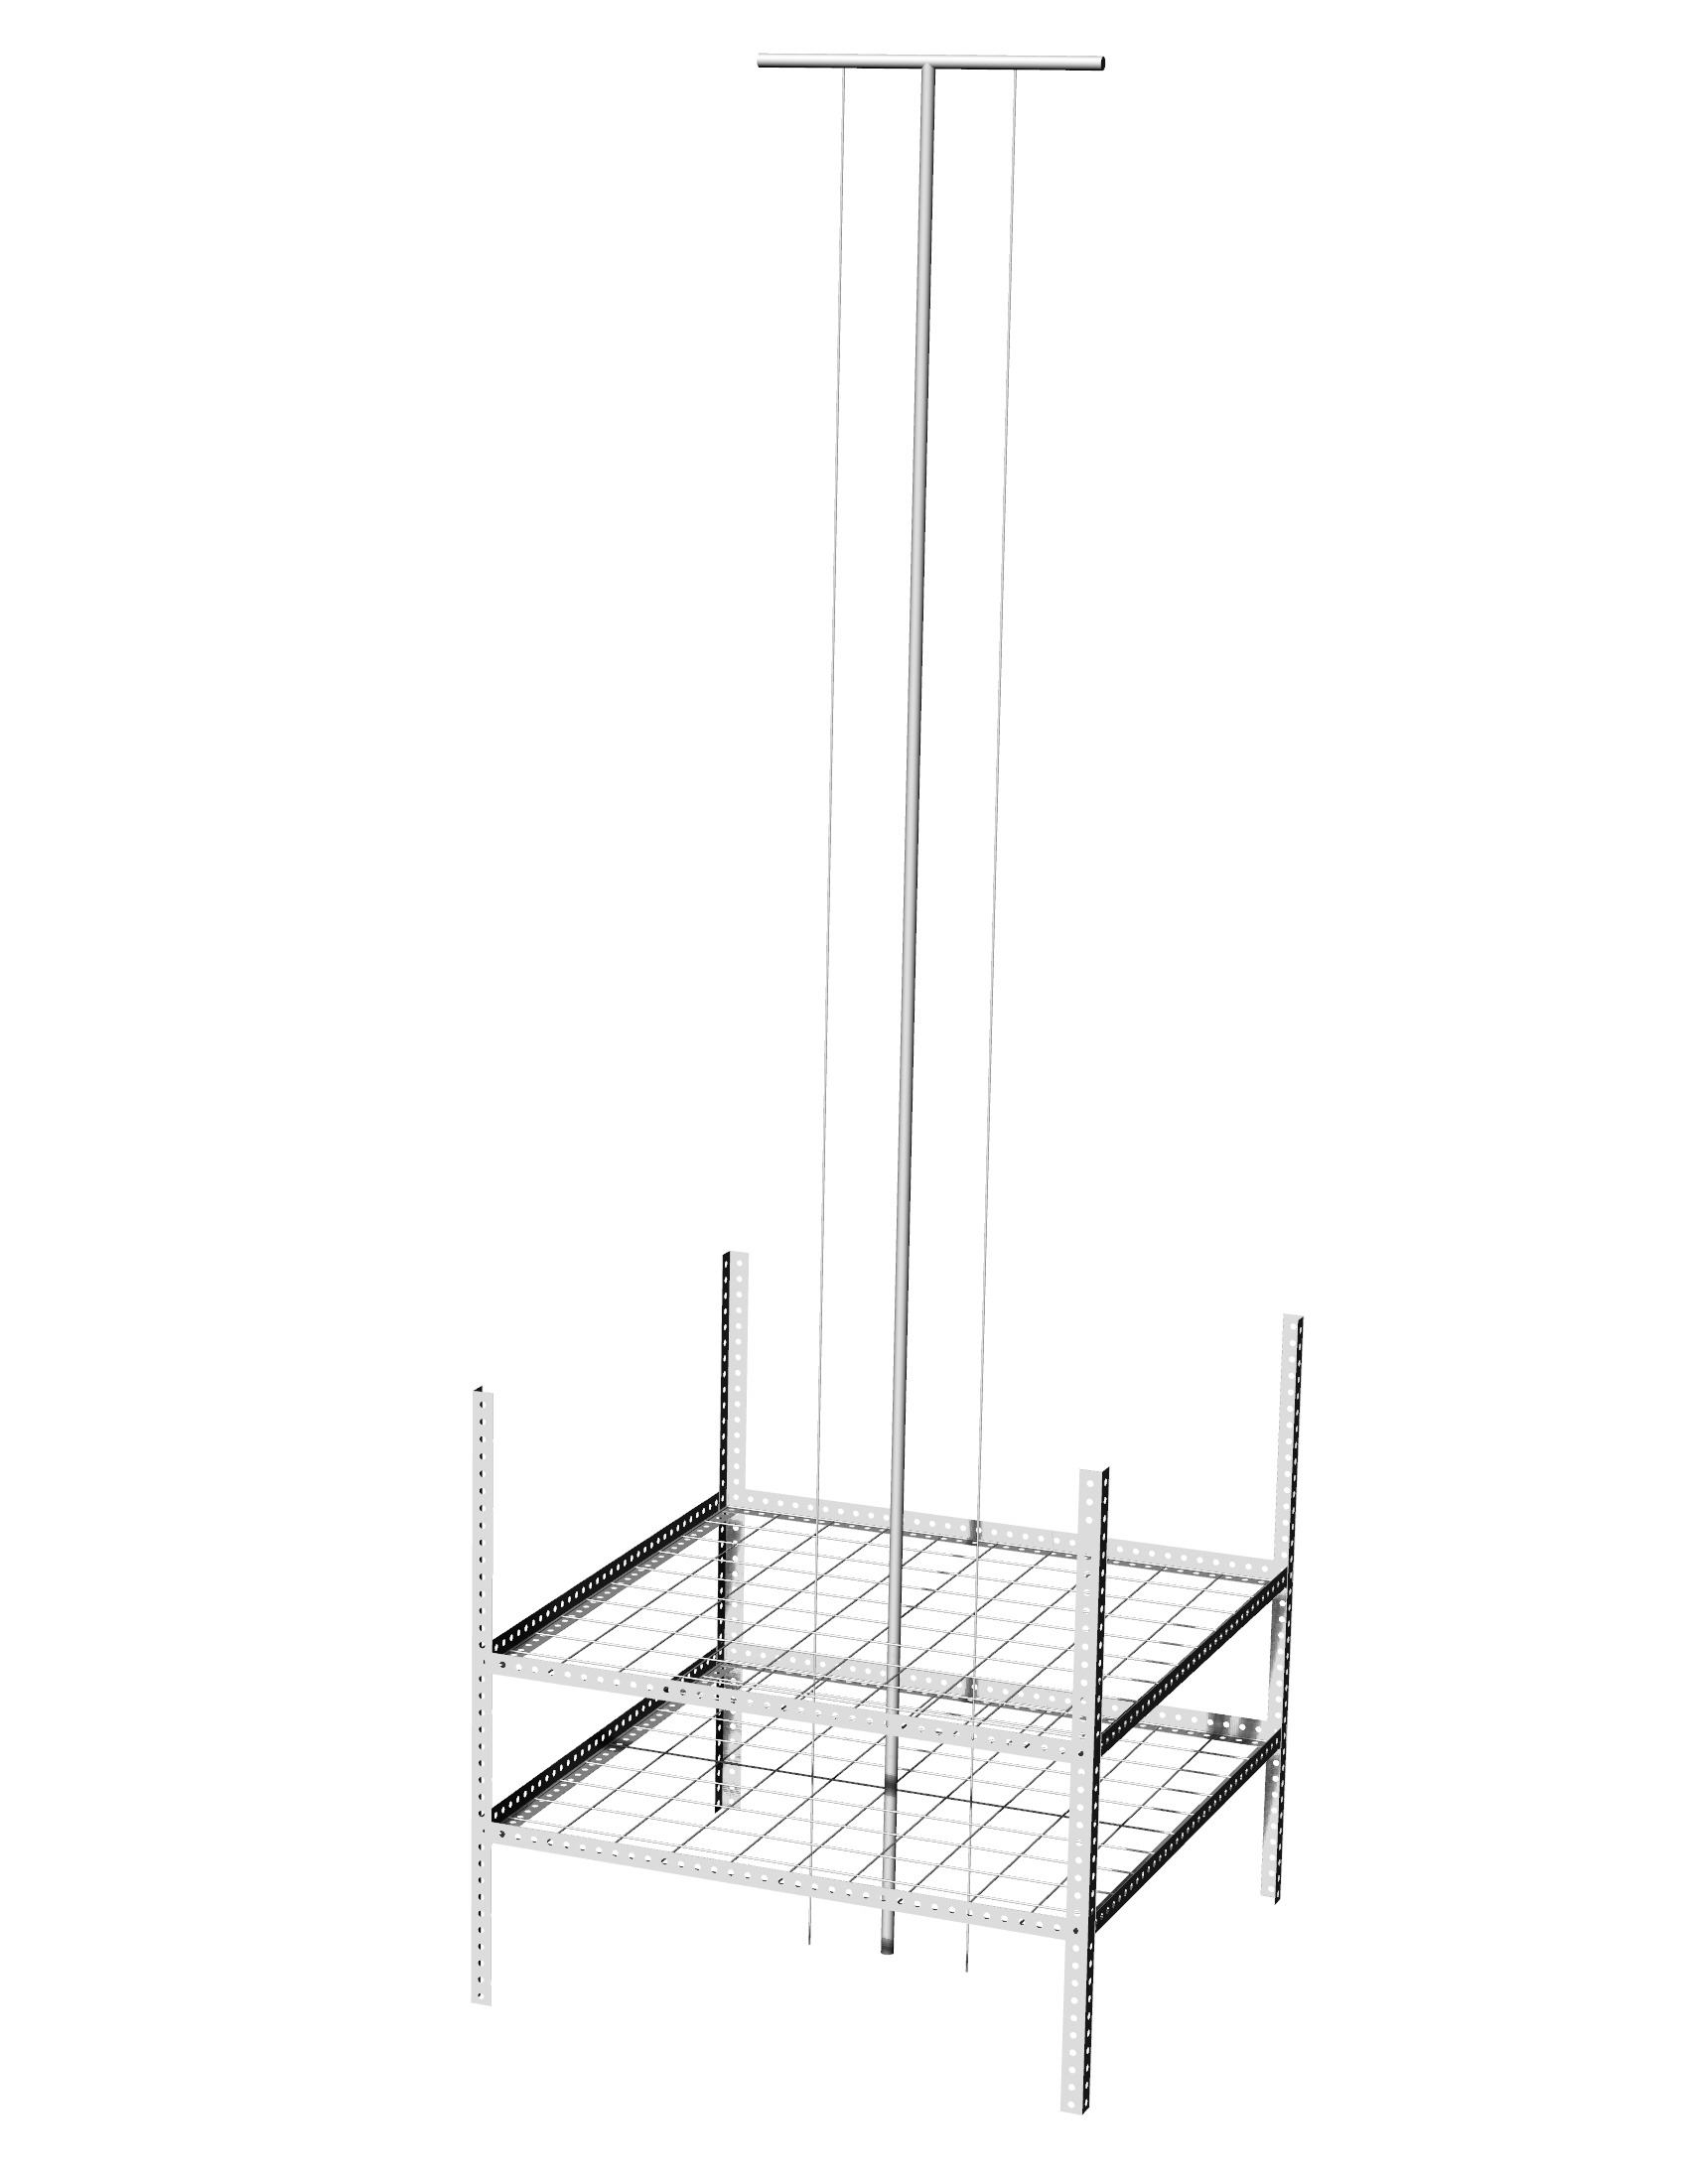
\includegraphics{figures/FABIOdraft.jpg}

\hypertarget{data-collection-and-analysis}{%
\subsection{Data collection and
analysis}\label{data-collection-and-analysis}}

Our experimental design was to conduct six burns, three piled and three
standing, for each of five fuel loads (250 g, 500 g, 1000 g, 1500 g,
2000 g) spanning the range of cogongrass biomass observed from field
measurements across Florida, USA.

Thermocouple sensor specs Thermocouple logger specs

Weather data was recorded at a two second interval during fires using a
Kestrel 5500 Fire Weather Pro pocket weather tracker (Nielsen-Kellerman,
Boothwyn, PA) mounted on a tripod to be \textasciitilde{}1 m above the
ground.

We used linear regression to model the average maximum temperature and
time above 100 ºC at each probe height, and the average flame height,
rate of spread, and percent consumed from each fire. Fuel load (mass)
and fuel structure (piled vs.~standing) were used as explanatory
variables, with fuel load treated as continuous. We tested the main
effects and interaction of these variables. If the interaction did not
have a strong effect we fit a new model with only main effects. We
report results from models that

We applied a linear model where

\[
y_{i} = \alpha + \beta_{1}*biomass_{i} + \beta_{2}*biomass_{i}*structure_{i}
\]

\begin{verbatim}
      date               fire_id         fabio_id      biomass    
 Min.   :2017-12-01   Min.   :43.00   Min.   :1.0   Min.   : 250  
 1st Qu.:2017-12-03   1st Qu.:50.75   1st Qu.:1.0   1st Qu.: 500  
 Median :2017-12-04   Median :58.50   Median :1.5   Median :1000  
 Mean   :2017-12-03   Mean   :58.50   Mean   :1.5   Mean   :1047  
 3rd Qu.:2017-12-05   3rd Qu.:66.25   3rd Qu.:2.0   3rd Qu.:1500  
 Max.   :2017-12-05   Max.   :74.00   Max.   :2.0   Max.   :2000  
                                                                  
 litter_biomass   pct_green   biomass_type        structure        
 Min.   :0      Min.   : NA   Length:32          Length:32         
 1st Qu.:0      1st Qu.: NA   Class :character   Class :character  
 Median :0      Median : NA   Mode  :character   Mode  :character  
 Mean   :0      Mean   :NaN                                        
 3rd Qu.:0      3rd Qu.: NA                                        
 Max.   :0      Max.   : NA                                        
                NA's   :32                                         
 rate_of_spread_50cm f_litter_biomass    f_biomass         total_biomass 
 Min.   : 0.000      Length:32          Length:32          Min.   : 250  
 1st Qu.: 6.287      Class :character   Class :character   1st Qu.: 500  
 Median :22.110      Mode  :character   Mode  :character   Median :1000  
 Mean   :30.946                                            Mean   :1047  
 3rd Qu.:48.797                                            3rd Qu.:1500  
 Max.   :95.660                                            Max.   :2000  
                                                                         
  pct_consumed    est_pct_fuel_moisture pct_fuel_moisture  max_flame_ht  
 Min.   : 22.84   Min.   : 0.000        Min.   : 4.634    Min.   :  0.0  
 1st Qu.: 96.90   1st Qu.: 7.171        1st Qu.: 9.453    1st Qu.: 54.5  
 Median : 99.11   Median : 9.457        Median :10.947    Median : 75.5  
 Mean   : 90.38   Mean   : 9.693        Mean   :11.494    Mean   :102.6  
 3rd Qu.: 99.58   3rd Qu.:13.310        3rd Qu.:13.978    3rd Qu.:170.0  
 Max.   :100.00   Max.   :18.399        Max.   :19.576    Max.   :256.0  
                  NA's   :3                                              
  avg_flame_ht     max_fuel_ht     avg_litter_depth  avg_green_ht    
 Min.   :  0.00   Min.   :  7.00   Min.   :0        Min.   :  4.667  
 1st Qu.: 38.12   1st Qu.: 15.75   1st Qu.:0        1st Qu.: 14.083  
 Median : 64.00   Median : 82.00   Median :0        Median : 76.333  
 Mean   : 87.31   Mean   : 84.22   Mean   :0        Mean   : 79.438  
 3rd Qu.:138.25   3rd Qu.:151.25   3rd Qu.:0        3rd Qu.:143.833  
 Max.   :248.00   Max.   :177.00   Max.   :0        Max.   :164.000  
                                                                     
  avg_brown_ht  avg_fuel_ht     
 Min.   : NA   Min.   :  4.667  
 1st Qu.: NA   1st Qu.: 14.083  
 Median : NA   Median : 76.333  
 Mean   :NaN   Mean   : 79.438  
 3rd Qu.: NA   3rd Qu.:143.833  
 Max.   : NA   Max.   :164.000  
 NA's   :32                     
\end{verbatim}

\begin{verbatim}
   location          structure            fire_id         max_temp     
 Length:96          Length:96          Min.   :43.00   Min.   : 40.26  
 Class :character   Class :character   1st Qu.:50.75   1st Qu.:244.32  
 Mode  :character   Mode  :character   Median :58.50   Median :366.70  
                                       Mean   :58.50   Mean   :371.79  
                                       3rd Qu.:66.25   3rd Qu.:540.18  
                                       Max.   :74.00   Max.   :773.88  
                                                                       
 avg2_max_temp       s_abv100     heat_flux_abv100  
 Min.   : 40.13   Min.   :  2.0   Min.   :   206.3  
 1st Qu.:241.09   1st Qu.: 57.5   1st Qu.: 12995.4  
 Median :357.98   Median : 91.0   Median : 19776.9  
 Mean   :363.49   Mean   :131.4   Mean   : 32289.4  
 3rd Qu.:525.23   3rd Qu.:139.0   3rd Qu.: 36001.6  
 Max.   :749.66   Max.   :824.0   Max.   :295967.4  
                  NA's   :13      NA's   :13        
\end{verbatim}

\begin{longtable}[]{@{}ccccccc@{}}
\caption{Summary of weather for each fire (means ± SE). Fire IDs 54, 56,
70, \& 74 were assigned values from their paired fires 53, 55, 69, \& 73
due to missing data.}\tabularnewline
\toprule
Fire ID & Date & Structure & Biomass & Air temperature (ºC) & RH (\%) &
Wind Speed (m s\textsuperscript{-1})\tabularnewline
\midrule
\endfirsthead
\toprule
Fire ID & Date & Structure & Biomass & Air temperature (ºC) & RH (\%) &
Wind Speed (m s\textsuperscript{-1})\tabularnewline
\midrule
\endhead
43 & 2017-12-01 & piled & 250 & 27.88 ± 0.08 & 36.8 ± 0.08 & 0.88 ±
0.08\tabularnewline
44 & 2017-12-01 & standing & 250 & 28.11 ± 0.09 & 36.33 ± 0.1 & 0.84 ±
0.09\tabularnewline
45 & 2017-12-01 & piled & 500 & 27.82 ± 0.09 & 37.51 ± 0.05 & 0.38 ±
0.09\tabularnewline
46 & 2017-12-01 & standing & 500 & 27.82 ± 0.09 & 37.2 ± 0.06 & 0.43 ±
0.09\tabularnewline
47 & 2017-12-01 & piled & 1000 & 22.81 ± 0.02 & 64.44 ± 0.06 & 0 ±
0.02\tabularnewline
48 & 2017-12-01 & standing & 1000 & 26.08 ± 0.02 & 44.83 ± 0.12 & 0.35 ±
0.02\tabularnewline
49 & 2017-12-01 & piled & 1500 & 22.27 ± 0.03 & 67.71 ± 0.05 & 0 ±
0.03\tabularnewline
50 & 2017-12-01 & standing & 1500 & 22.76 ± 0.02 & 65.97 ± 0.06 & 0 ±
0.02\tabularnewline
51 & 2017-12-04 & piled & 2000 & 26.69 ± 0.06 & 55.88 ± 0.13 & 0.58 ±
0.06\tabularnewline
52 & 2017-12-04 & standing & 2000 & 28.21 ± 0.15 & 54.27 ± 0.23 & 0.44 ±
0.15\tabularnewline
53 & 2017-12-04 & piled & 250 & 25.75 ± 0.04 & 55.15 ± 0.12 & 0.02 ±
0.04\tabularnewline
54 & 2017-12-04 & standing & 250 & 25.75 ± 0.04 & 55.15 ± 0.12 & 0.02 ±
0.04\tabularnewline
55 & 2017-12-04 & piled & 500 & 25.26 ± 0.06 & 57.39 ± 0.14 & 0.25 ±
0.06\tabularnewline
56 & 2017-12-04 & standing & 500 & 25.26 ± 0.06 & 57.39 ± 0.14 & 0.25 ±
0.06\tabularnewline
57 & 2017-12-04 & piled & 1000 & 24.25 ± 0.04 & 60.04 ± 0.1 & 0.37 ±
0.04\tabularnewline
58 & 2017-12-04 & standing & 1000 & 23.57 ± 0.01 & 61.57 ± 0.1 & 0.77 ±
0.01\tabularnewline
59 & 2017-12-04 & piled & 1000 & 25.38 ± 0.04 & 59.71 ± 0.09 & 0.1 ±
0.04\tabularnewline
60 & 2017-12-04 & standing & 1000 & 25.79 ± 0.04 & 58.32 ± 0.15 & 0 ±
0.04\tabularnewline
61 & 2017-12-04 & piled & 2000 & 24.3 ± 0.01 & 63.52 ± 0.15 & 0 ±
0.01\tabularnewline
62 & 2017-12-04 & standing & 2000 & 24.2 ± 0 & 62.53 ± 0.01 & 0 ±
0\tabularnewline
63 & 2017-12-05 & piled & 250 & 26.91 ± 0.05 & 60.61 ± 0.08 & 1.09 ±
0.05\tabularnewline
64 & 2017-12-05 & standing & 250 & 27.08 ± 0.09 & 60.48 ± 0.06 & 1.1 ±
0.09\tabularnewline
65 & 2017-12-05 & piled & 500 & 28.71 ± 0.09 & 56.63 ± 0.13 & 0.72 ±
0.09\tabularnewline
66 & 2017-12-05 & standing & 500 & 29.28 ± 0.15 & 55.86 ± 0.2 & 0.69 ±
0.15\tabularnewline
67 & 2017-12-05 & piled & 1000 & 28.22 ± 0.1 & 55.96 ± 0.21 & 0.49 ±
0.1\tabularnewline
68 & 2017-12-05 & standing & 1000 & 27.72 ± 0.1 & 56.96 ± 0.14 & 0.59 ±
0.1\tabularnewline
69 & 2017-12-05 & piled & 1500 & 27.11 ± 0.05 & 59.57 ± 0.08 & 1.02 ±
0.05\tabularnewline
70 & 2017-12-05 & standing & 1500 & 27.11 ± 0.05 & 59.57 ± 0.08 & 1.02 ±
0.05\tabularnewline
71 & 2017-12-05 & piled & 2000 & 28.47 ± 0.06 & 52.05 ± 0.11 & 0.71 ±
0.06\tabularnewline
72 & 2017-12-05 & standing & 2000 & 28.35 ± 0.17 & 52.16 ± 0.09 & 0.43 ±
0.17\tabularnewline
73 & 2017-12-05 & piled & 1500 & 30.33 ± 0.01 & 47.63 ± 0.02 & 0 ±
0.01\tabularnewline
74 & 2017-12-05 & standing & 1500 & 30.33 ± 0.01 & 47.63 ± 0.02 & 0 ±
0.01\tabularnewline
\bottomrule
\end{longtable}

\hypertarget{fuel-moisture}{%
\subsubsection{Fuel moisture}\label{fuel-moisture}}

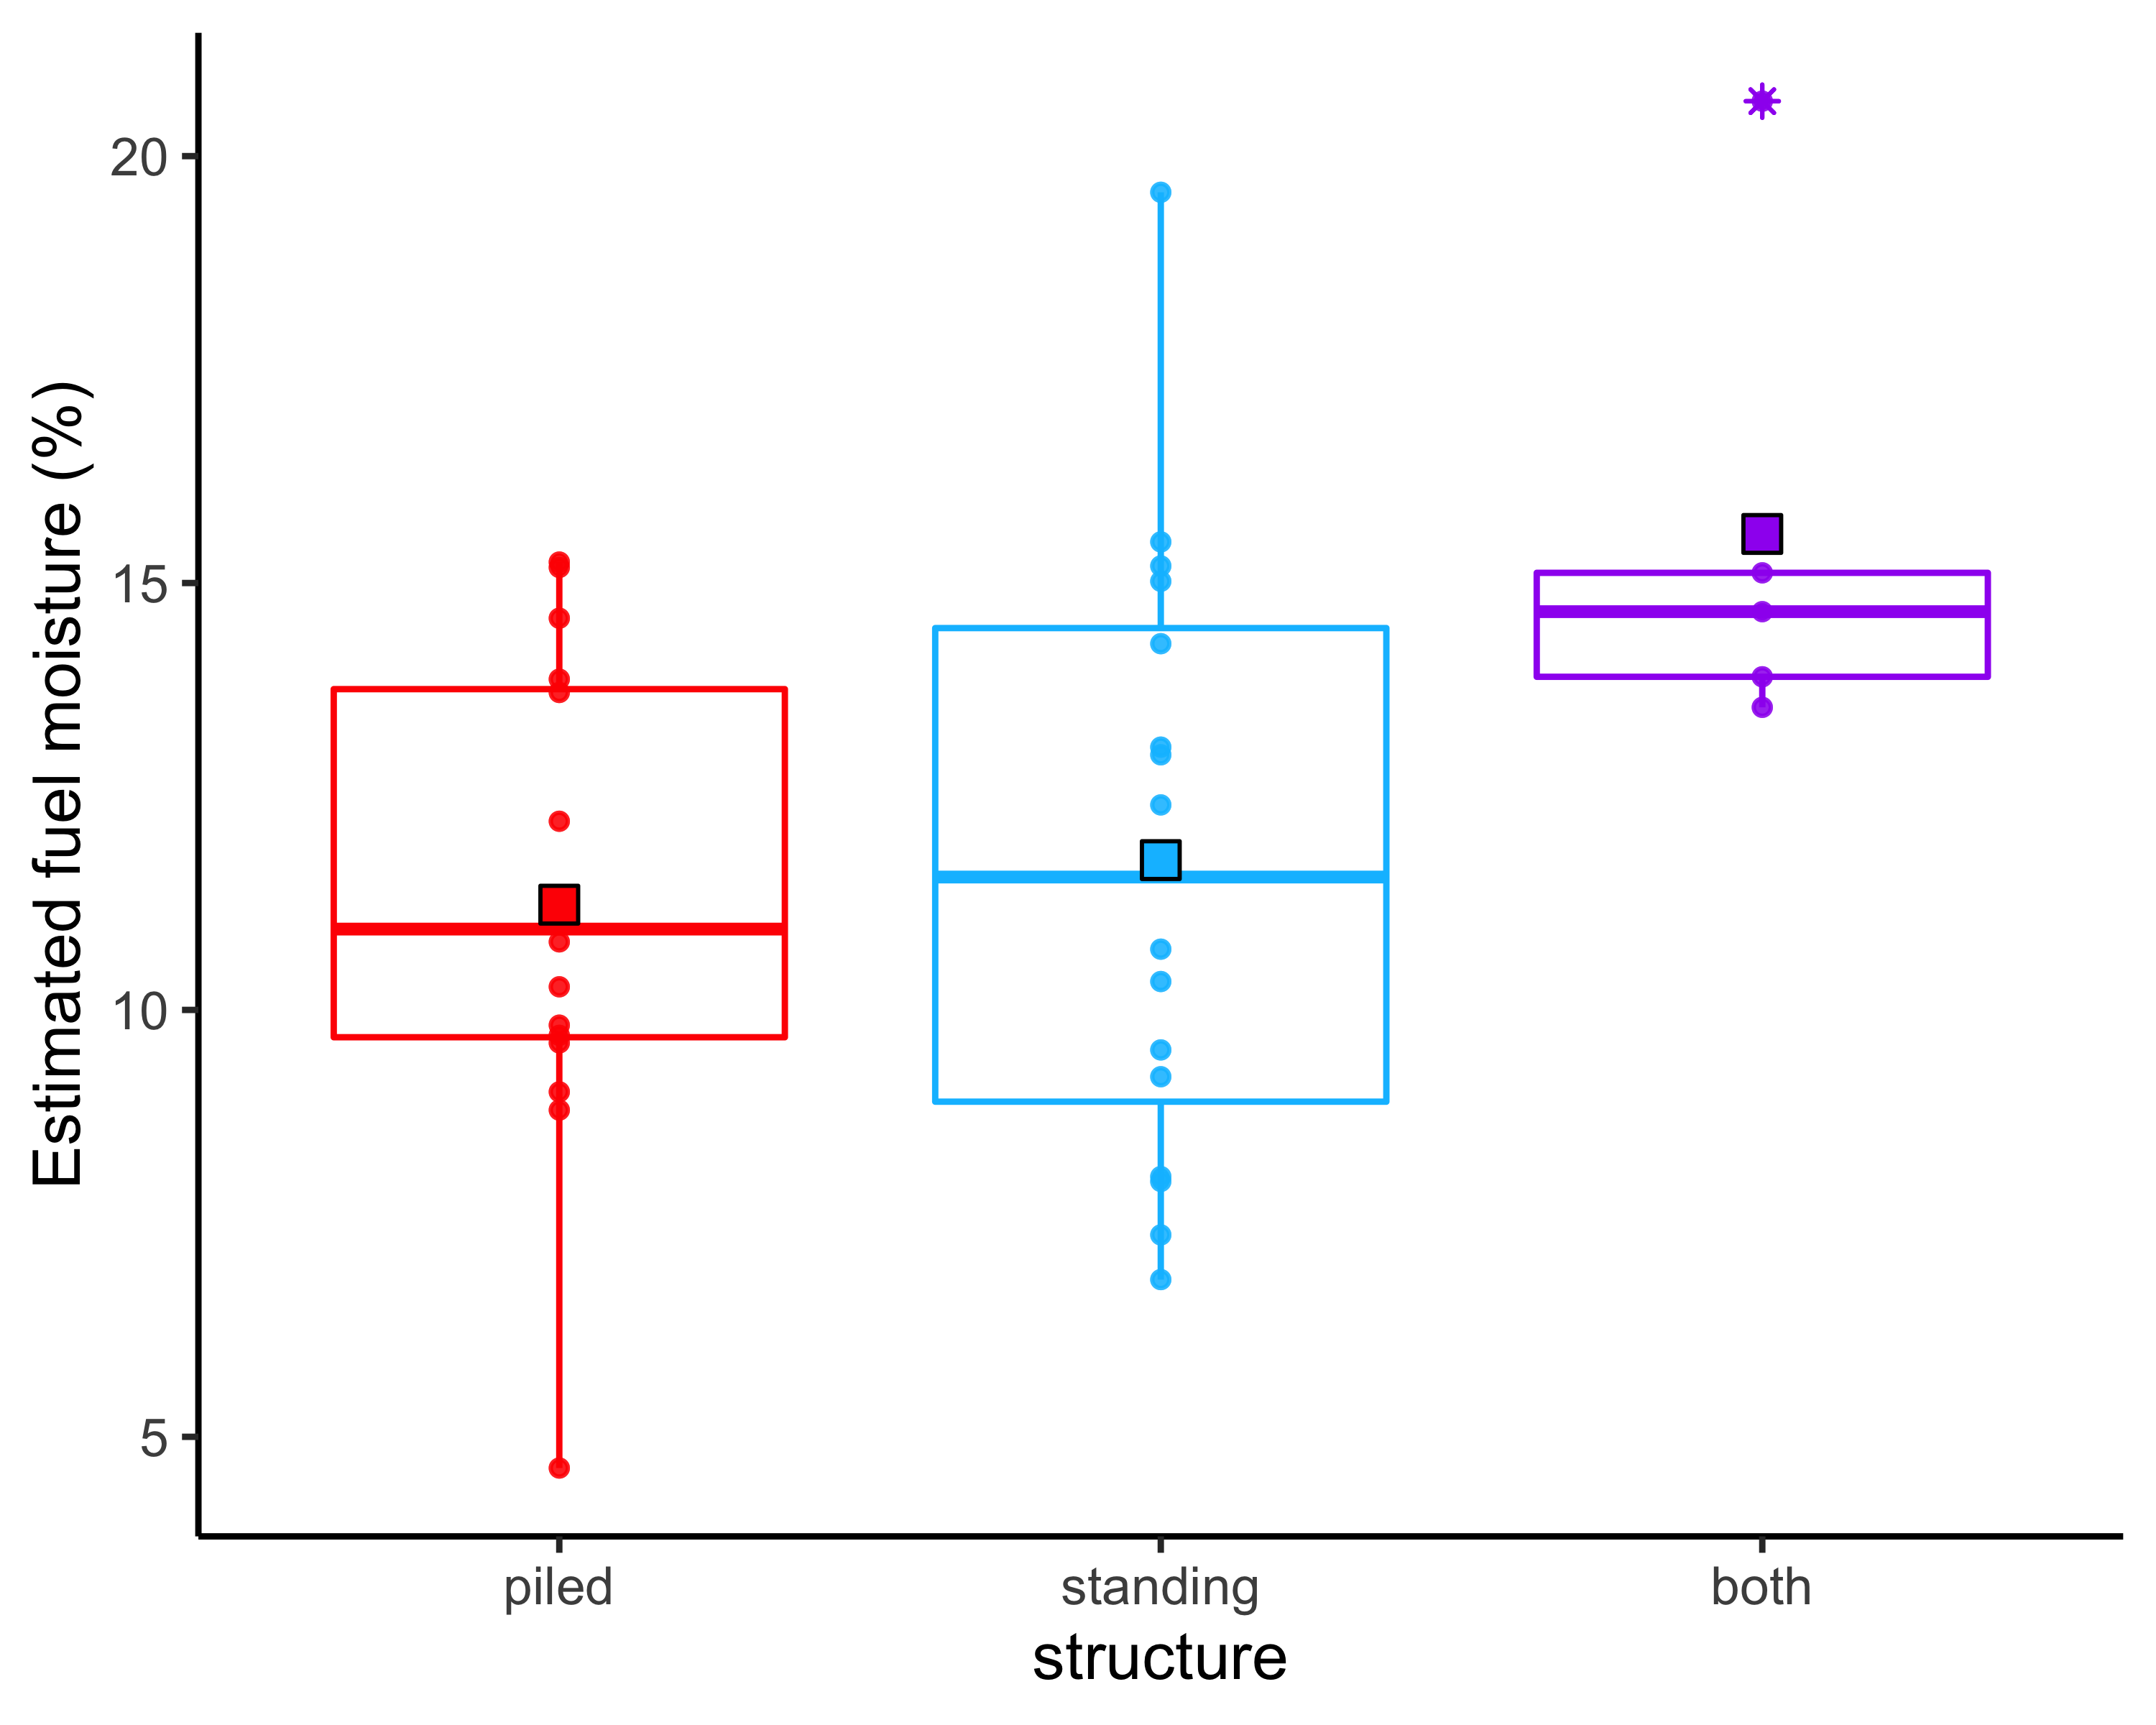
\includegraphics{figures/fuel_moisture-1.png}

Across all fires fuel moisture content ranged from 4.6 to 19.6\% (mean =
11.49±0.56\%).

\hypertarget{linear-models-of-maximum-temperature}{%
\subsubsection{Linear models of maximum
temperature}\label{linear-models-of-maximum-temperature}}

The ``maximum temperature'' at each height is the average of the maximum
temperatures from the three temperature probes located at that height.
For some of the fires with the lowest amount of biomass (250 g) the
probe temperature did not deviate from near-ambient (Fig. 3).

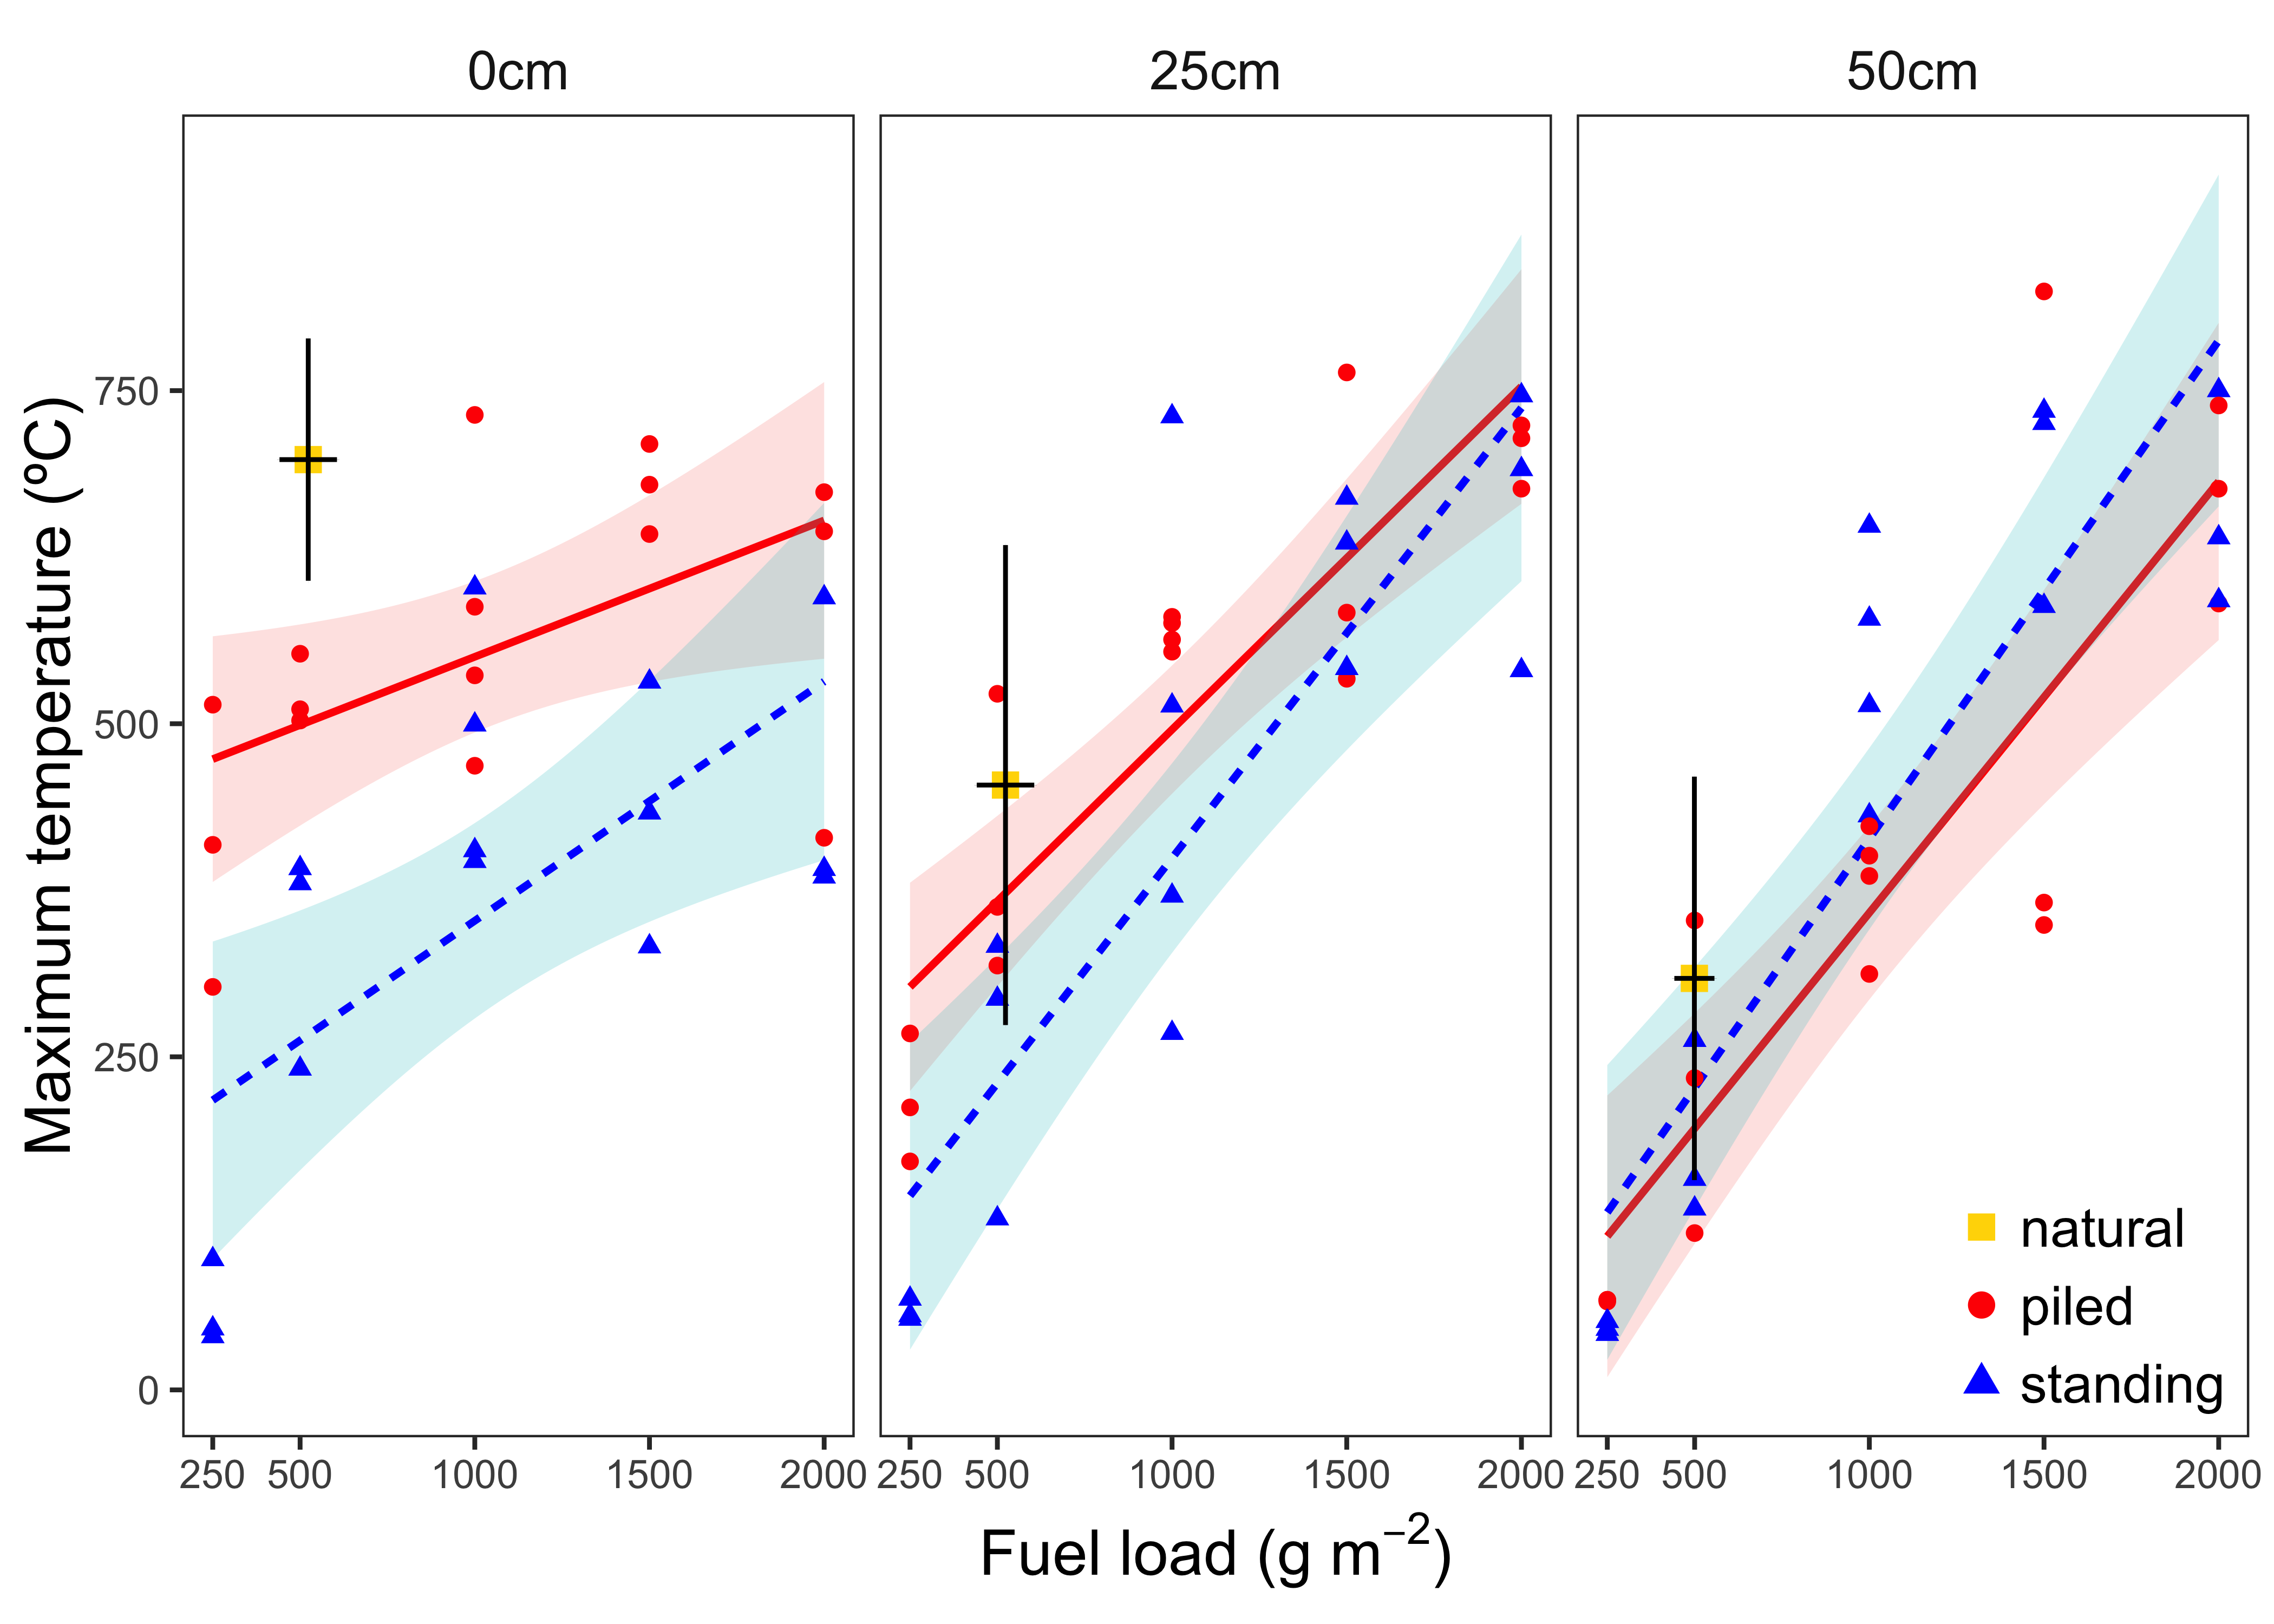
\includegraphics{figures/maxtemp-figure-1.png}

\begin{verbatim}

Call:
lm(formula = max_temp ~ biomass * structure, data = fabio_fires_0cm)

Residuals:
    Min      1Q  Median      3Q     Max 
-163.21 -115.29   15.26   90.02  287.15 

Coefficients:
                            Estimate Std. Error t value Pr(>|t|)    
(Intercept)                384.52101   57.12710   6.731 2.62e-07 ***
biomass                      0.07345    0.04695   1.564   0.1290    
structurestanding         -255.90652   80.78992  -3.168   0.0037 ** 
biomass:structurestanding    0.11008    0.06640   1.658   0.1085    
---
Signif. codes:  0 '***' 0.001 '**' 0.01 '*' 0.05 '.' 0.1 ' ' 1

Residual standard error: 116.5 on 28 degrees of freedom
Multiple R-squared:  0.5122,    Adjusted R-squared:  0.4599 
F-statistic:   9.8 on 3 and 28 DF,  p-value: 0.0001381
\end{verbatim}

\begin{verbatim}

Call:
lm(formula = max_temp ~ biomass + structure, data = fabio_fires_0cm)

Residuals:
    Min      1Q  Median      3Q     Max 
-215.66  -81.21    4.56   86.92  284.57 

Coefficients:
                    Estimate Std. Error t value Pr(>|t|)    
(Intercept)        326.90139   46.68516   7.002 1.06e-07 ***
biomass              0.12849    0.03419   3.759 0.000767 ***
structurestanding -140.66729   42.39658  -3.318 0.002451 ** 
---
Signif. codes:  0 '***' 0.001 '**' 0.01 '*' 0.05 '.' 0.1 ' ' 1

Residual standard error: 119.9 on 29 degrees of freedom
Multiple R-squared:  0.4643,    Adjusted R-squared:  0.4274 
F-statistic: 12.57 on 2 and 29 DF,  p-value: 0.0001173
\end{verbatim}

\begin{longtable}[]{@{}lrrrrrr@{}}
\caption{Max temperature at ground level}\tabularnewline
\toprule
& Estimate & Std. Error & t value &
Pr(\textgreater{}\textbar{}t\textbar{}) & 2.5 \% & 97.5
\%\tabularnewline
\midrule
\endfirsthead
\toprule
& Estimate & Std. Error & t value &
Pr(\textgreater{}\textbar{}t\textbar{}) & 2.5 \% & 97.5
\%\tabularnewline
\midrule
\endhead
(Intercept) & 326.901 & 46.685 & 7.002 & 0.000 & 231.420 &
422.383\tabularnewline
Biomass & 0.128 & 0.034 & 3.759 & 0.001 & 0.059 & 0.198\tabularnewline
Structure: standing & -140.667 & 42.397 & -3.318 & 0.002 & -227.378 &
-53.957\tabularnewline
\bottomrule
\end{longtable}

\begin{verbatim}

Call:
lm(formula = max_temp ~ biomass * structure, data = fabio_fires_25cm)

Residuals:
    Min      1Q  Median      3Q     Max 
-172.18  -64.49  -24.20   51.38  365.91 

Coefficients:
                            Estimate Std. Error t value Pr(>|t|)    
(Intercept)                166.52310   54.42279   3.060  0.00484 ** 
biomass                      0.21240    0.04473   4.749 5.51e-05 ***
structurestanding         -140.67599   76.96544  -1.828  0.07826 .  
biomass:structurestanding    0.11911    0.06326   1.883  0.07013 .  
---
Signif. codes:  0 '***' 0.001 '**' 0.01 '*' 0.05 '.' 0.1 ' ' 1

Residual standard error: 110.9 on 28 degrees of freedom
Multiple R-squared:  0.735, Adjusted R-squared:  0.7066 
F-statistic: 25.88 on 3 and 28 DF,  p-value: 3.172e-08
\end{verbatim}

\begin{verbatim}

Call:
lm(formula = max_temp ~ biomass + structure, data = fabio_fires_25cm)

Residuals:
    Min      1Q  Median      3Q     Max 
-145.20  -94.76  -13.18   56.47  363.11 

Coefficients:
                   Estimate Std. Error t value Pr(>|t|)    
(Intercept)       104.17636   45.04802   2.313    0.028 *  
biomass             0.27195    0.03299   8.244 4.33e-09 ***
structurestanding -15.98250   40.90984  -0.391    0.699    
---
Signif. codes:  0 '***' 0.001 '**' 0.01 '*' 0.05 '.' 0.1 ' ' 1

Residual standard error: 115.7 on 29 degrees of freedom
Multiple R-squared:  0.7014,    Adjusted R-squared:  0.6808 
F-statistic: 34.06 on 2 and 29 DF,  p-value: 2.447e-08
\end{verbatim}

\begin{longtable}[]{@{}lrrrrrr@{}}
\caption{Max temperature at 25cm}\tabularnewline
\toprule
& Estimate & Std. Error & t value &
Pr(\textgreater{}\textbar{}t\textbar{}) & 2.5 \% & 97.5
\%\tabularnewline
\midrule
\endfirsthead
\toprule
& Estimate & Std. Error & t value &
Pr(\textgreater{}\textbar{}t\textbar{}) & 2.5 \% & 97.5
\%\tabularnewline
\midrule
\endhead
(Intercept) & 104.176 & 45.048 & 2.313 & 0.028 & 12.043 &
196.310\tabularnewline
Biomass & 0.272 & 0.033 & 8.244 & 0.000 & 0.204 & 0.339\tabularnewline
Structure: standing & -15.982 & 40.910 & -0.391 & 0.699 & -99.653 &
67.688\tabularnewline
\bottomrule
\end{longtable}

\begin{verbatim}

Call:
lm(formula = max_temp ~ biomass * structure, data = fabio_fires_50cm)

Residuals:
     Min       1Q   Median       3Q      Max 
-157.851  -54.343   -5.386   28.149  190.955 

Coefficients:
                           Estimate Std. Error t value Pr(>|t|)    
(Intercept)                24.65978   42.18178   0.585   0.5635    
biomass                     0.25062    0.03467   7.229  7.2e-08 ***
structurestanding         -12.08180   59.65404  -0.203   0.8410    
biomass:structurestanding   0.11922    0.04903   2.432   0.0217 *  
---
Signif. codes:  0 '***' 0.001 '**' 0.01 '*' 0.05 '.' 0.1 ' ' 1

Residual standard error: 85.99 on 28 degrees of freedom
Multiple R-squared:  0.8653,    Adjusted R-squared:  0.8508 
F-statistic: 59.94 on 3 and 28 DF,  p-value: 2.631e-12
\end{verbatim}

\begin{longtable}[]{@{}lrrrrrr@{}}
\caption{Max temperature at 50cm}\tabularnewline
\toprule
& Estimate & Std. Error & t value &
Pr(\textgreater{}\textbar{}t\textbar{}) & 2.5 \% & 97.5
\%\tabularnewline
\midrule
\endfirsthead
\toprule
& Estimate & Std. Error & t value &
Pr(\textgreater{}\textbar{}t\textbar{}) & 2.5 \% & 97.5
\%\tabularnewline
\midrule
\endhead
(Intercept) & 24.660 & 42.182 & 0.585 & 0.563 & -61.746 &
111.065\tabularnewline
Biomass & 0.251 & 0.035 & 7.229 & 0.000 & 0.180 & 0.322\tabularnewline
Structure: standing & -12.082 & 59.654 & -0.203 & 0.841 & -134.278 &
110.114\tabularnewline
Biomass*Standing & 0.119 & 0.049 & 2.432 & 0.022 & 0.019 &
0.220\tabularnewline
\bottomrule
\end{longtable}

\hypertarget{time-above-100-c-figure}{%
\subsubsection{Time above 100 ºC figure}\label{time-above-100-c-figure}}

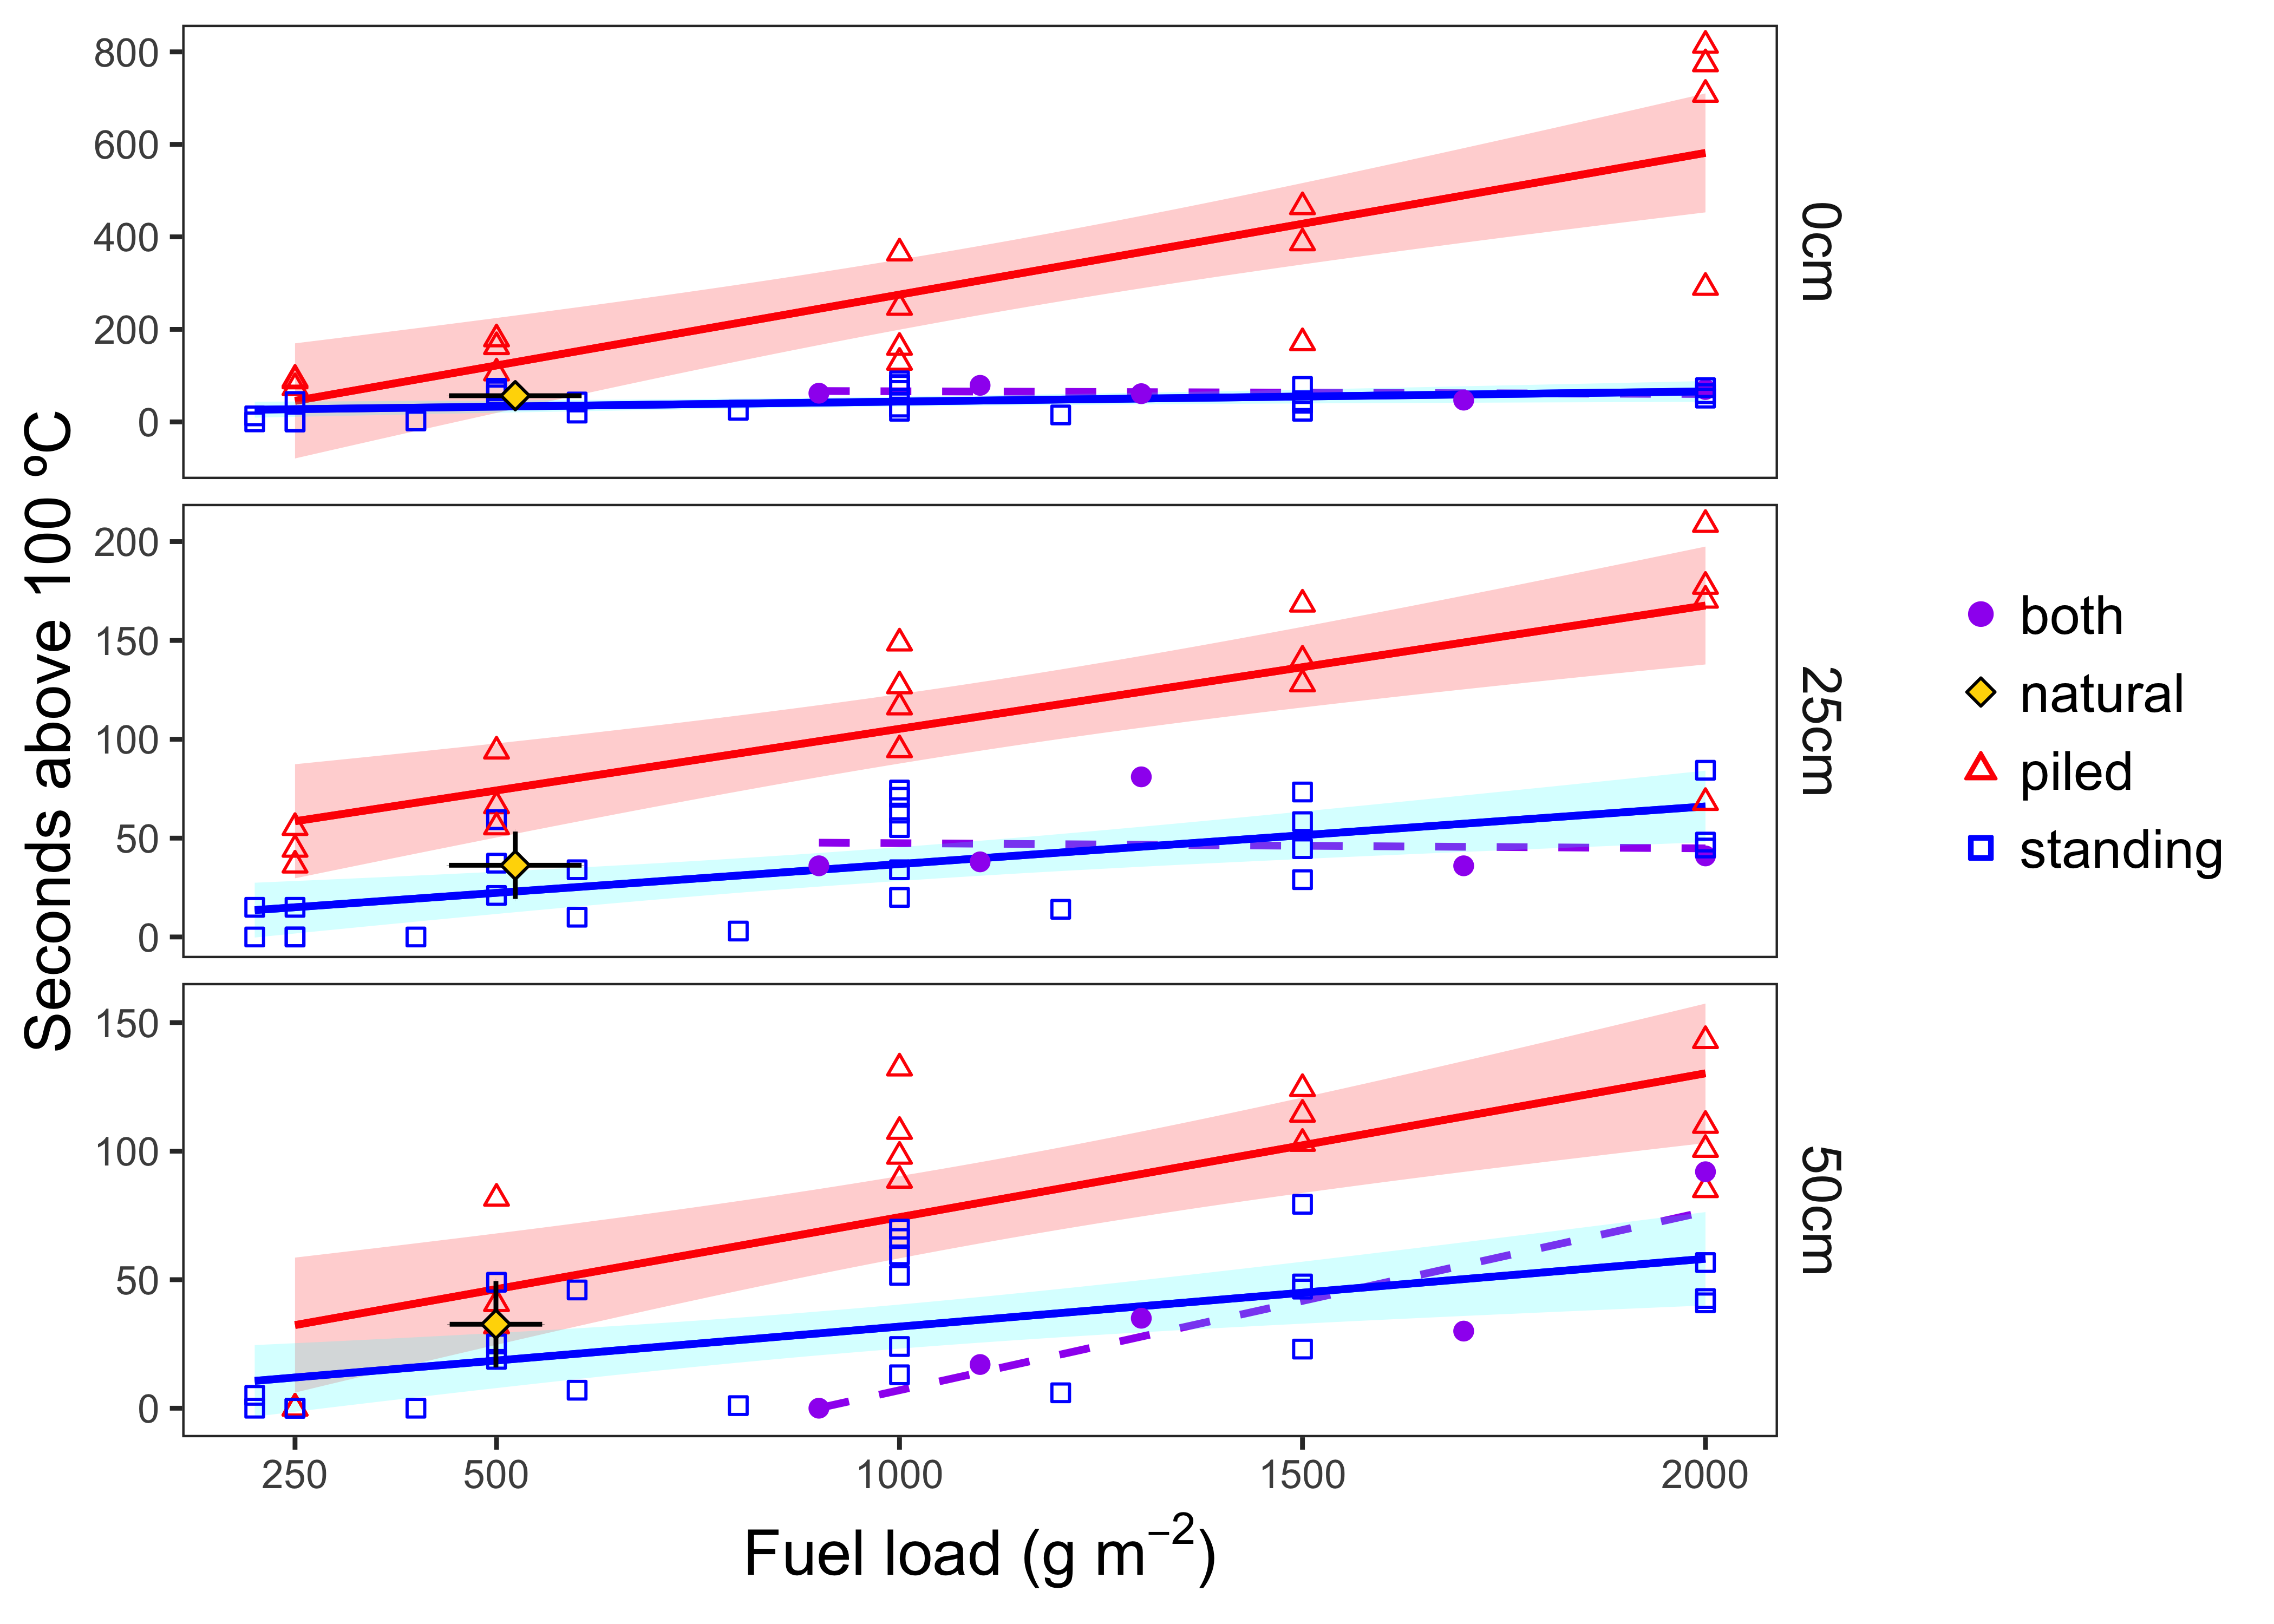
\includegraphics{figures/compare_secsAbv100-1.png}

\begin{longtable}[]{@{}lrrrr@{}}
\caption{Time above 100 ºC (seconds) at ground level}\tabularnewline
\toprule
& Estimate & Std. Error & t value &
Pr(\textgreater{}\textbar{}t\textbar{})\tabularnewline
\midrule
\endfirsthead
\toprule
& Estimate & Std. Error & t value &
Pr(\textgreater{}\textbar{}t\textbar{})\tabularnewline
\midrule
\endhead
(Intercept) & 135.401 & 51.289 & 2.640 & 0.013\tabularnewline
Biomass & 0.159 & 0.038 & 4.225 & 0.000\tabularnewline
Strcture: standing & -240.375 & 46.578 & -5.161 & 0.000\tabularnewline
\bottomrule
\end{longtable}

\begin{longtable}[]{@{}lrrrr@{}}
\caption{Time above 100 ºC (seconds) at 25cm}\tabularnewline
\toprule
& Estimate & Std. Error & t value &
Pr(\textgreater{}\textbar{}t\textbar{})\tabularnewline
\midrule
\endfirsthead
\toprule
& Estimate & Std. Error & t value &
Pr(\textgreater{}\textbar{}t\textbar{})\tabularnewline
\midrule
\endhead
(Intercept) & 71.616 & 14.910 & 4.803 & 0\tabularnewline
Biomass & 0.060 & 0.011 & 5.491 & 0\tabularnewline
Strcture: standing & -83.625 & 13.541 & -6.176 & 0\tabularnewline
\bottomrule
\end{longtable}

\begin{longtable}[]{@{}lrrrr@{}}
\caption{Time above 100 ºC (seconds) at 50cm}\tabularnewline
\toprule
& Estimate & Std. Error & t value &
Pr(\textgreater{}\textbar{}t\textbar{})\tabularnewline
\midrule
\endfirsthead
\toprule
& Estimate & Std. Error & t value &
Pr(\textgreater{}\textbar{}t\textbar{})\tabularnewline
\midrule
\endhead
(Intercept) & 36.168 & 15.452 & 2.341 & 0.026\tabularnewline
Biomass & 0.054 & 0.011 & 4.740 & 0.000\tabularnewline
Strcture: standing & -50.500 & 14.033 & -3.599 & 0.001\tabularnewline
\bottomrule
\end{longtable}

\includegraphics{figures/unnamed-chunk-2-1.png}

\hypertarget{flame-height-figure}{%
\subsubsection{Flame height figure}\label{flame-height-figure}}

\includegraphics{figures/flame height fig-1.png}

\hypertarget{biomass-consumed-figure}{%
\subsubsection{Biomass consumed figure}\label{biomass-consumed-figure}}

\includegraphics{figures/compare biomass consumption-1.png}

\hypertarget{rate-of-spread-figure}{%
\subsubsection{Rate of spread figure}\label{rate-of-spread-figure}}

Rate of spread was measured by recording the number of seconds it took
the fire-line to travel 50 cm and then converted to units of m
s\textsuperscript{-1}.

\includegraphics{figures/rate_of_spread-1.png}

We used the statistical language \texttt{R} (R Core Team 2018) for all
our analyses. These were implemented in dynamic rmarkdown documents
using \texttt{knitr} (Xie 2014, 2015, 2018) and \texttt{rmarkdown}
(Allaire et al. 2018) packages. All the multilevel models were fitted
with \texttt{lme4} (Bates et al. 2015).

\hypertarget{results}{%
\section{RESULTS}\label{results}}

Trees in forest A grew taller than those in forest B (mean height: 25
versus 13 m). And many more cool results that get updated dynamically.

\hypertarget{discussion}{%
\section{DISCUSSION}\label{discussion}}

Discuss.

\hypertarget{conclusions}{%
\section{CONCLUSIONS}\label{conclusions}}

\hypertarget{acknowledgements}{%
\section{ACKNOWLEDGEMENTS}\label{acknowledgements}}

\hypertarget{references}{%
\section{REFERENCES}\label{references}}

\hypertarget{refs}{}
\leavevmode\hypertarget{ref-Allaire_2018}{}%
Allaire, J., Y. Xie, J. McPherson, J. Luraschi, K. Ushey, A. Atkins, H.
Wickham, J. Cheng, and W. Chang. 2018. Rmarkdown: Dynamic documents for
r.

\leavevmode\hypertarget{ref-Bates_2015}{}%
Bates, D., M. Mächler, B. Bolker, and S. Walker. 2015. Fitting linear
mixed-effects models using lme4. Journal of Statistical Software
67:1--48.

\leavevmode\hypertarget{ref-Bowman2017}{}%
Bowman, D. M. J. S., C. Haverkamp, K. D. Rann, and L. D. Prior. 2017.
Differential demographic filtering by surface fires: How fuel type and
fuel load affect sapling mortality of an obligate seeder savanna tree.
Journal of Ecology:1--13.

\leavevmode\hypertarget{ref-Fernandes2012}{}%
Fernandes, P. M., and M. G. Cruz. 2012. Plant flammability experiments
offer limited insight into vegetation-fire dynamics interactions. New
Phytologist 194:606--609.

\leavevmode\hypertarget{ref-JAUREGUIBERRY2011}{}%
JAUREGUIBERRY, P., G. BERTONE, and S. DÍAZ. 2011. Device for the
standard measurement of shoot flammability in the field. Austral Ecology
36:821--829.

\leavevmode\hypertarget{ref-Loudermilk2014}{}%
Loudermilk, E. L., G. L. Achtemeier, J. J. O'brien, J. K. Hiers, and B.
S. Hornsby. 2014. High-resolution observations of combustion in
heterogeneous surface fuels. International Journal of Wildland Fire
23:1016--1026.

\leavevmode\hypertarget{ref-R_Core_Team_2018}{}%
R Core Team. 2018. R: A language and environment for statistical
computing. R Foundation for Statistical Computing, Vienna, Austria.

\leavevmode\hypertarget{ref-Simpson2016}{}%
Simpson, K. J., B. S. Ripley, P. A. Christin, C. M. Belcher, C. E.
Lehmann, G. H. Thomas, and C. P. Osborne. 2016. Determinants of
flammability in savanna grass species. Journal of Ecology 104:138--148.

\leavevmode\hypertarget{ref-Thaxton2006}{}%
Thaxton, J. M., and W. J. Platt. 2006. Small-scale fuel variation alters
fire intensity and shrub abundance in a pine savanna. Ecology
87:1331--1337.

\leavevmode\hypertarget{ref-Wyse2016}{}%
Wyse, S. V., G. L. Perry, D. M. O'Connell, P. S. Holland, M. J. Wright,
C. L. Hosted, S. L. Whitelock, I. J. Geary, K. J. Maurin, and T. J.
Curran. 2016. A quantitative assessment of shoot flammability for 60
tree and shrub species supports rankings based on expert opinion.
International Journal of Wildland Fire 25:466--477.

\leavevmode\hypertarget{ref-Xie_2014}{}%
Xie, Y. 2014. Knitr: A comprehensive tool for reproducible research in
R. \emph{in} V. Stodden, F. Leisch, and R. D. Peng, editors.
Implementing reproducible computational research. Chapman; Hall/CRC.

\leavevmode\hypertarget{ref-Xie_2015}{}%
Xie, Y. 2015. Dynamic documents with R and knitr. 2nd editions. Chapman;
Hall/CRC, Boca Raton, Florida.

\leavevmode\hypertarget{ref-Xie_2018}{}%
Xie, Y. 2018. Knitr: A general-purpose package for dynamic report
generation in r.

\eleft

\clearpage


\listoftables


\newpage

\begin{longtable}[]{@{}rrrrl@{}}
\caption{A glimpse of the famous \emph{Iris} dataset.}\tabularnewline
\toprule
Sepal.Length & Sepal.Width & Petal.Length & Petal.Width &
Species\tabularnewline
\midrule
\endfirsthead
\toprule
Sepal.Length & Sepal.Width & Petal.Length & Petal.Width &
Species\tabularnewline
\midrule
\endhead
5.1 & 3.5 & 1.4 & 0.2 & setosa\tabularnewline
4.9 & 3.0 & 1.4 & 0.2 & setosa\tabularnewline
4.7 & 3.2 & 1.3 & 0.2 & setosa\tabularnewline
4.6 & 3.1 & 1.5 & 0.2 & setosa\tabularnewline
5.0 & 3.6 & 1.4 & 0.2 & setosa\tabularnewline
5.4 & 3.9 & 1.7 & 0.4 & setosa\tabularnewline
\bottomrule
\end{longtable}

\newpage



\clearpage

\listoffigures


\newpage

\includegraphics{figures/Fig2_3panel.pdf} \newpage

\newpage

\includegraphics{figures/timeandmaxtempPanels2x2.pdf}

\newpage

\blandscape

\begin{figure}
\centering
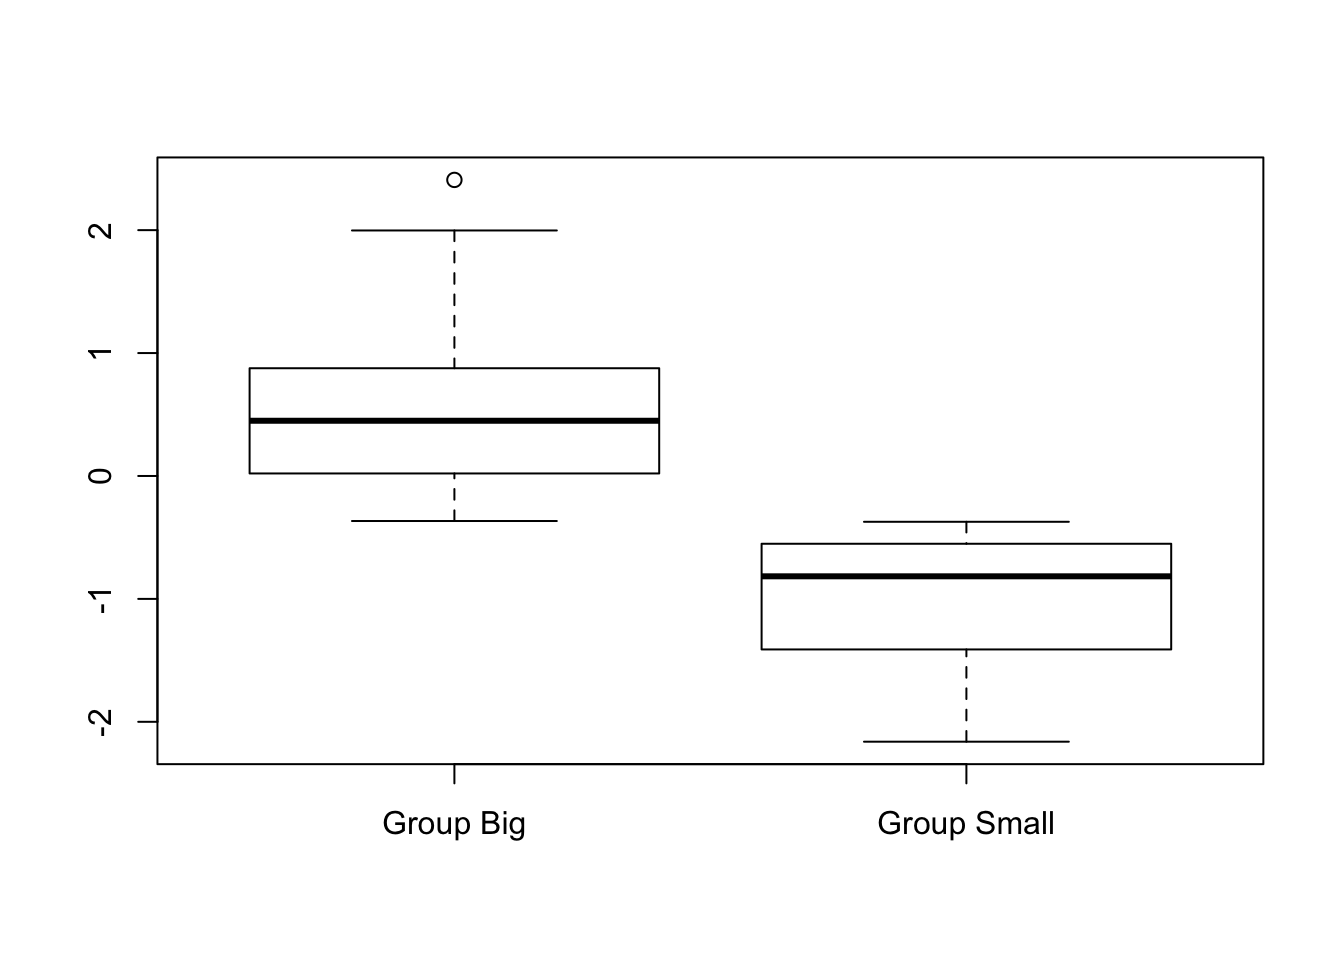
\includegraphics{figures/Fig2-1.png}
\caption{Second figure in landscape format.}
\end{figure}

\elandscape

\clearpage

\hypertarget{key-experimental-fire-ecology-studies-for-reference}{%
\subsection{Key experimental fire ecology studies for
reference}\label{key-experimental-fire-ecology-studies-for-reference}}

(Bowman et al. 2017) \emph{Differential demographic filtering by surface
fires: How fuel type and fuel load affect sapling mortality of an
obligate seeder savanna tree.}

In this study, ``Grass fuels had to be laid horizontally rather than
standing vertically.'' The context provided is that the native sorghum
grass flattens easily after it dries and does not remain vertical
throughout the dry season.

\begin{itemize}
\item
  This reads like a response to a reviewer comment, which might indicate
  a gap that the FABIO methodology can fill.
\item
  Average flame height was measured ``when the fire was within 15cm of
  the tree stem using a metal grid placed verically against a steel
  picket placed next to the stem.''
\end{itemize}

Additional references given where fuels have been laid flat when testing
flammability:

\begin{itemize}
\item
  \textbf{({\textbf{???}})}

  \begin{itemize}
  \item
    Built the ``Bar-B-Q''" apparatus to fill a need to quantify
    flammability of whole plants of many species
  \item
    Quantified flammability characteristics of 34 species using ``whole
    plant''
  \item
    Fuels are still burnt horizontally, so no vertical structure
  \item
    Length of fuel limited by size of burning surface
  \end{itemize}
\item
  \textbf{(Simpson et al. 2016)}

  \begin{itemize}
  \item
    Assessed flammability of 25 savanna grass species
  \item
    five plant traits: biomass quantity, biomass density, biomass
    moisture content, leaf surface-area:volume ratio, leaf effective
    heat combustion
  \item
    related plant traits to three components of flammability:
    ignitability, sustainability, combustibility at leaf and plant
    scales
  \item
    Results: total above-ground biomass drove combustibility and
    sustainability - high biomass was more intense for longer; moisture
    content was main driver of ignitability and also reduced combustion
    rate; estimates of whole-plant combustion rates showed
    \textgreater{}20-fold variation; Showed that there was significant
    variation between species in flammability at the plant-level and
    leaf-level
  \end{itemize}
\item
  \textbf{(Wyse et al. 2016)}
\end{itemize}

\emph{All of these studies assessed flammability of multiple species, or
multiple fuel complexes.}

\end{document}